\chapter{LQR Controller}

\section{Introduction}

After validating the PID controller, the TA asked if it would be possible to design another controller able to only use
the second motor when the first one struggles to reach the desired speed. This desire suits to the system as the motor 2
is weaker than the first one: it can be seen easily as its time constant $\tau$ is greater than the one of motor 1, 
meaning that it needs more time to reach a set value.

\section{State Space Model}
In control system design, it is often easier to define a parameterized state-space model in continuous time because 
physical laws are typically described using differential equations. The linear state-space representation in 
continuous-time has the following form:

\begin{equation}
    \dot{\mathbf{x}} = A \mathbf{x} + B \mathbf{u}
    \label{eq:state_space_models}
\end{equation}

where \( \mathbf{x} \) is the state vector, \( A \) is the state matrix that represents the system dynamics, 
\( B \) is the input matrix that represents the control input, and \( \mathbf{u} \) is the input vector.\\
To get to the state space representation from the transfer function is quite easy as each motor is a $1^{st}$ order
system. By using the following property of the Laplace transform:

\begin{align}
    X(s) &= \mathcal{L}\left\{x(t)\right\}\\
    s X(s) &= \mathcal{L}\left\{\frac{d x(t)}{dt}\right\}
\end{align}

The transfer function \ref{eq:1_st_order_TF} can be put in the temporal domain:

\begin{gather}
    G(s) = \frac{Y(s)}{U(s)} = \frac{A_0}{\tau s + 1}\\
    \left(\tau s + 1\right) Y(s) = A_0 U(s)\\
    \tau \dot{y}(t) + y(t) = A_0 u(t)\\
    \dot{y}(t) = \frac{-1}{\tau} y(t) + \frac{A_0}{\tau} u(t)
\end{gather}

This can be done for both motors with respectively ($u_1/y_1$) and ($u_2/y_2$) as input and output. With the choice of 
state $x_i(t) = y_i(t)$, the state space representation becomes

\begin{equation}
    \dot{\mathbf{x}}(t) = \begin{bmatrix}
    \frac{-1}{\tau_1} & 0 \\ 
    0 & \frac{-1}{\tau_2}
    \end{bmatrix} \mathbf{x}(t) + \begin{bmatrix} 
    \frac{A_{01}}{\tau_1} & 0\\ 
    0 & \frac{A_{02}}{\tau_2} 
    \end{bmatrix}\mathbf{u}(t)
    \label{eq:state_space_model_cx}
\end{equation}

\begin{equation}
    y(t) = \begin{bmatrix} 1 & 1 \end{bmatrix}\mathbf{x}(t)
    \label{eq:state_space_model_cy}
\end{equation}

where \( y \) is the velocity output, which is just the sum of both imposed speeds ($y = y_1 + y_2$).

\section{Discrete-Time State-Space Model}
We convert the continuous-time state-space model \eqref{eq:state_space_model_cx} and \eqref{eq:state_space_model_cy} to 
a discrete-time state-space model using the parameters from the identification section (\ref{section:identification}):

\[
\tau_1 = 1.915, \quad \tau_2 = 1.7, \quad A_{01} = 24.88, \quad A_{02} = 19.51.
\]

The continuous-time matrices are computed as:

\[
\mathbf{A} = 
\begin{bmatrix}
-0.5218 & 0 \\
0 & -0.5882
\end{bmatrix}, \quad 
\mathbf{B} = 
\begin{bmatrix}
12.9870 & 0\\
0 & 11.4765
\end{bmatrix}.
\]

For a sampling time \( T_s = 0.005 \, \text{seconds} \), the discrete-time matrices \( A_{T_s} \) and \( B_{T_s} \) are calculated as follows:

\begin{itemize}
    \item \textbf{Discrete-Time State Matrix} (\(A_{T_s}\)): 
   Using the matrix exponential formula:
   \[
   A_{T_s} = e^{A T_s},
   \]
   where:
   \[
   A T_s = 
   \begin{bmatrix}
   -0.002609 & 0 \\
   0 & -0.002941
   \end{bmatrix}.
   \]
   Since \( A T_s \) is a diagonal matrix, the matrix exponential is computed as:

   \begin{gather*}
        e^{A T_s} = \begin{bmatrix} e^{-0.002609} & 0 \\ 0 & e^{-0.002941} \end{bmatrix}\\
        A_{T_s} = \begin{bmatrix} 0.9974 & 0 \\ 0 & 0.9971 \end{bmatrix}
   \end{gather*}

\end{itemize}


\begin{itemize} 
    \item \textbf{Discrete-Time Input Matrix} (\(B_{T_s}\)): 
   Using the formula:
   \[
   B_{T_s} = \int_0^{T_s} e^{A \zeta} B \, d\zeta,
   \]
   and solving numerically, we find:
   \[
   B_{T_s} = 
   \begin{bmatrix}
    0.0647 & 0\\
    0 & 0.0570
   \end{bmatrix}.
   \]
\end{itemize}

Thus, the discrete-time state-space representation of the system is:

\begin{gather*}
    x[k+1] = 
        \begin{bmatrix} 0.9974 & 0 \\ 0 & 0.9971 \end{bmatrix} x[k] 
    + \begin{bmatrix} 0.0647 & 0\\ 0 & 0.0570 \end{bmatrix} u[k]\\
    y[k] = \begin{bmatrix} 1 & 1 \end{bmatrix} x[k]
\end{gather*}



Finally, the sampled system is equivalent to a discrete-time system with these matrices. We will now use this representation to design an LQR controller for the given discrete-time system.

\section{Controller design}

To build a state feedback regulator, two steps must be completed. First, an observer has to be built to derive the state of 
the system from the input and the output of it. Then, the state feedback control law must be determined.\\
The design of those two parts (observer and state feedback) can be done independently thanks to the separation 
principle. The structure of the whole controller will be:

\begin{figure}[H]
    \centering
    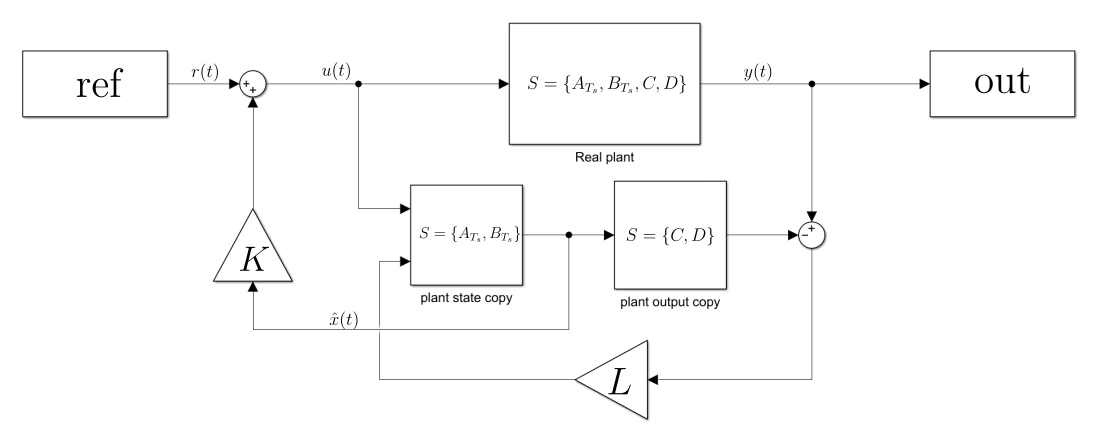
\includegraphics[width = \textwidth]{Pictures/lqr_controller.png}
    \caption{Structure of the LQR controller}
    \label{fig:lqr structure}
\end{figure}

\subsection{Observer}

The observer will consist of a copy of the system and a feedback as shown in fig \ref{fig:observer structure}. In this
section, the matrix $L$ must be determined in a way such that the resulting observer is asymptotic.

\begin{figure}[H]
    \centering
    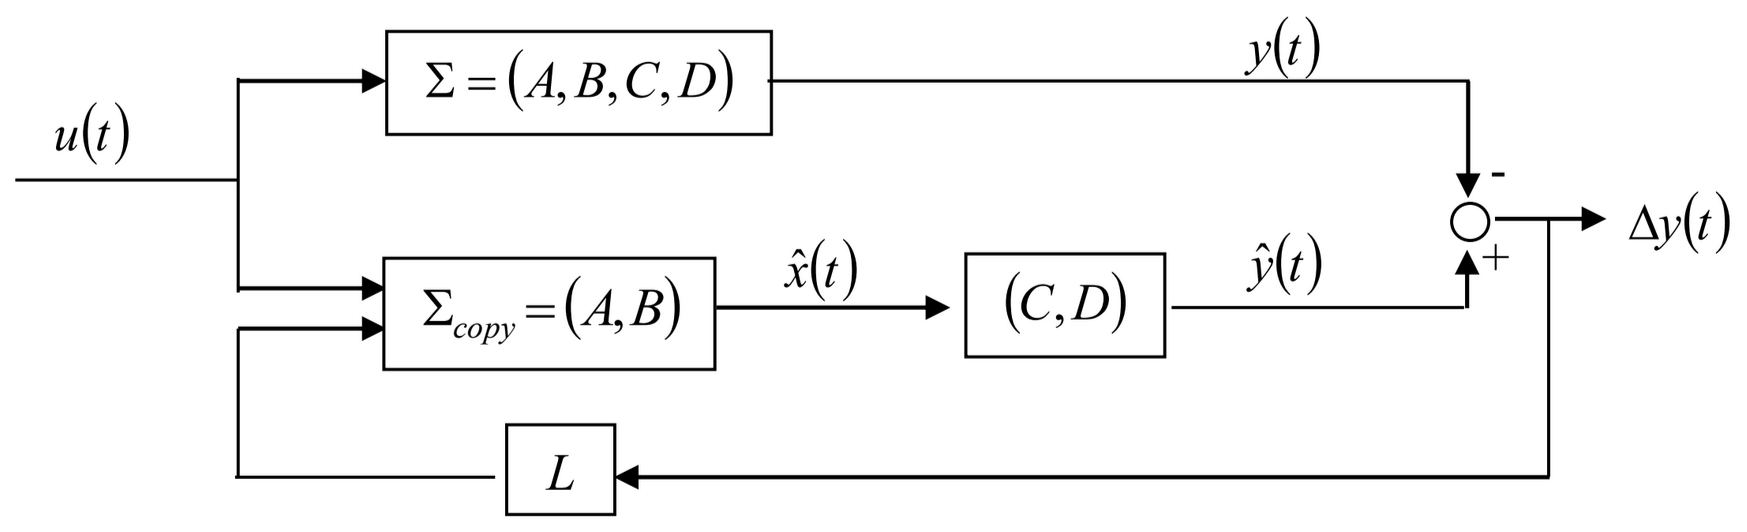
\includegraphics[height=\textheight/7]{Pictures/observer_general_structure.png}
    \caption{Generic structure of an observer}
    \label{fig:observer structure}
\end{figure}

For an observer to be asymptotic, the eigenvalues of $(A + LC)$ must be converging. It is however important to not skip
a step in the design. First, the observability matrix $\mathcal{O}_2$ of the system must be computed:

\begin{equation}
    \mathcal{O}_2 = 
    \begin{bmatrix}
        C\\
        C A_{T_s}
    \end{bmatrix}
    =
    \begin{bmatrix}
        1 & 1\\
        0.9974 & 0.9971
    \end{bmatrix}
\end{equation}

Now that we are sure that $\mathcal{O}_2$ is full rank, we can conclude that the system is detectable and that a matrix
L that will make the observer asymptotic exists. Because the state error $\hat{x}(t) - x(t)$ converges with 
$\lambda_i^t$\footnote{$\lambda_1$ and $\lambda_2$ being the eigenvalues of $A_{T_s} + LC$}, it is a smart choice to try to make
those $\lambda_i$ close to 0.

\begin{gather}
    L = \begin{bmatrix} l_1\\l_2 \end{bmatrix}\\
    A_{T_s} + L C = \begin{bmatrix} 1+l_1 & 1+l_2 \\ 0.9974+l_1 & 0.9971+l_2 \end{bmatrix}
\end{gather}

An easy choice is $l_1 = -0.9974$ and $l_2 = -1$ to make $A_{T_s} + LC$ diagonal while ensuring that $\left|\lambda_i
\right| < 1$. This gives the final L matrix:

\begin{equation}
    L = \begin{bmatrix}
        -0.9974 \\ -1
    \end{bmatrix}
\end{equation}


\subsection{LQR Feedback Law}

To find a state feedback output law that corresponds to what we desire, the LQR method has been used.
The goal of the Linear Quadratic Regulator (LQR) is to minimize the quadratic cost function:

\[
J = \sum_{k=0}^\infty \left( x[k]^\top Q x[k] + u[k]^\top R u[k] \right).
\]

The weighting square matrices \( Q \) and \( R \) must be selected based on system requirements:

\begin{itemize}
    \item \( Q \): Penalizes state deviations, typically represented as a diagonal matrix, e.g., \( Q = \text{diag}(q_1, q_2) \).
    \item \( R \): Penalizes large control efforts, usually a positive scalar, \( R > 0 \).
\end{itemize}

For our design, $Q$ has been set to 1 because we don't care about state deviation. $R$ has been chosen such that the 
controller will prioritize the use of motor 1 over motor 2. 

\[
Q = 1, \quad
R = \begin{bmatrix}
1 & 0 \\
0 & 5
\end{bmatrix}.
\]

The optimal feedback gain matrix \( K \) is computed as:

\[
K = \left( R + B_{T_s}^\top P B_{T_s} \right)^{-1} \left(B_{T_s}^\top P A_{T_s} \right).
\]

Such that the controller state feedback will be:

\[
u[k] = -K \hat{x}[k] + r[k],
\]

where \( K \) is the gain matrix, $\hat{x}$ the estimated state from the observer and $r$ the reference to follow.

The computation results yield:

\[
K = \begin{bmatrix}
    0.9299 & 0\\
    0 & 0.3938
\end{bmatrix}
\]
